\chapter{Introduction}
\label{intro}

\section{Overview}
This project explores the use of identification and classification of food images for use in a calorie measurement android application.
Food calorie consumption is a huge problem in the modern world.
Over 25\% of the population in Ireland is obese and this figure is likely to rise over the coming years.
A mobile application that could help keep track of a user's calorie intake by taking pictures of their meals would be a great help.
The area of Machine Vision is a very difficult topic to address as it is a very hard task for computers to undertake.
We, as humans, take vision for granted as we can soon see, from the study of Machine Vision, that there are many difficult steps that have to be made for full identification and classification of an image.

When looking into calorie measurement using an image, there are three questions that have to be answered:
\begin{itemize}
\item{Where are the Regions of Interest (ROI) in this food image?}
\item{What food types are in these ROI's?}
\item{What is the portion size of each food type?}
\end{itemize}
In this project, my main focus will be on the first question, 'Where are the
Regions of Interest (ROI) in this food image?'. This is normally achieved
through image segmentation. Image segmentation is the process in which you
divide an image into multiple segments as per Figure \ref{fig:imageSeg} and \ref{fig:preImageSeg}.

\begin{figure}
	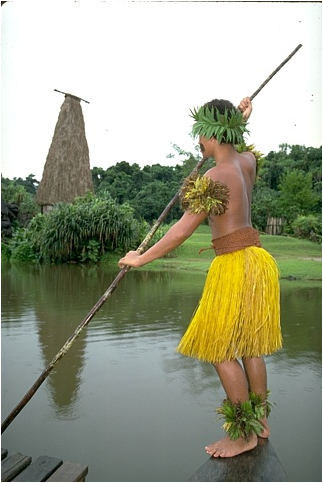
\includegraphics[scale=0.5]{orig}
	\caption{Pre-segmented Image}
	\label{fig:preImageSeg}
\end{figure}

\begin{figure}
	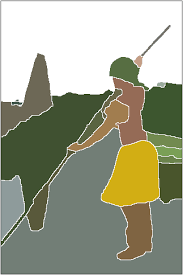
\includegraphics[scale=0.5]{segment}
	\caption{Segmented Image}
	\label{fig:imageSeg}
\end{figure}


Many researchers in various machine vision labs have attempted to solve this
problem using different methodologies.
There has been promising results from some papers but these are mostly under highly constrained circumstances.
When mixed foods are introduced to the problem, many of the methods fail.
Convolutional Neural Networks (CNN) have had very promising results in the field of image classification in the recent years but to get to the classification step, image segmentation is first needed, otherwise known as image identification.
Where CNN's have been shown to work best is in the area of face detection.

I have researched many different methods of image segmentation but it seems that CNN's have had the best results for multiple objects in one image and I hope to apply these results for many foods in an image.
This is because we will rarely want to classify an image that only has one food
item in it. Therefore, the one shot approach approach won't work by which we
build a classifier that takes in an image and gives back the most likely food in
that image.

The system that I am proposing to solve the problem statement would be able to
integrate with an Android mobile phone application.
The idea is, that when a user is about to eat their meal, they can simply take a picture of their meal for computation.
From here, the application would take the image, find the objects (ROI) in the image and take note of them.
Concurrently, the application would attempt to classify each object detected.
Once this is done, the size of each food type would be measured and through this an overall calorie count would be displayed for the user.
This could be logged for user metrics. 
I will focus on finding the objects for this application as I will not be able to implement the full system due to time constraints.

\section{Objectives}
\subsection*{Primary Objectives}
\subsubsection*{Use Convolutional Nueral Networks for Food Image Classification}
There has been a large paradigm shift in food image recognition in recent years to using convolutional nueral networks. I hope to use this paradigm to answer the problem statement.

\subsubsection*{Tune the CNN, replicating previous work}
There are many different approaches to food identification and classification,
many of which we will see in Chapter 2. I hope to select an approach that has
shown promising results in the past and replicate them. In addition to this, there are many different network architectures and parameters that can be adjused when building CNNs and I hope to tune these in order to get the best outcome I can.

\subsubsection*{Develop a mobile application to leverage the CNN}
Another objective for this project is to develop an application that can be used
for dietary assessment. This application would be able to take an image and then
identify and classify the foods within the image. I will not focus on size
estimation of the food type in this project.

\subsection*{Secondary Objectives}
\subsubsection*{Understanding of Convolutional Neural Networks}
In the project, I will be using Convolutional Neural Networks (CNN's) for object identification in Food Images.
I will be using an API for this due to time constraints but it is a key
objective for me to develop a deep understanding of CNN's as they are quite pivotal in the current Machine Vision Industry and I find bio-inspired systems very interesting.

\subsubsection*{Learn about different image identification and classification techniques}
Although, I will be using CNN's for my implementation, I will not be turning a
blind eye to other methods of identification and classification.
I have done extensive research on many different methods prior to my decision to use CNN's.
I think it is very important to learn about other methods as different methods
are better suited for some situations and it would be best to know about these methods due to the inevitability of their use.

\section{Methodology}
The following methodology were adapter for this project:

\subsection*{Define the research question}
The first step to this project was to define the research question.
I knew that I wanted to look into the general area of 'Food Identification and
Classification' but the scope of this is too broad for an FYP.
Therefore I decided that the research question would be to look at the food identification aspect ie. region of interest detection.

\subsection*{Literature Review}
Once I had defined the question, finding related work was the next milestone.
There are many attempts at Food Image Classification and these were not difficult to find, using Google Scholar, but many of these papers glossed over the segmentation aspect and relied on third parties for this step.
Because of this, I had to follow quite a few references to different papers that focused solely on image segmentation.

\subsection*{Explore different image identification methods}
I had collected various image identification methods from the literature review
that I carried out, so there were many options to evaluate.
I wanted to try something with Convolutional Neural Networks so more traditional
methods of identification using colour and texture was not so strenuously explored.

\subsection*{Select an image identification method}

\subsection*{Research technologies and develop skills in these technologies}
As I used a Convolutional Neural Network (CNN) in this project, I leveraged many resources to enrich my understanding of the process.
I decide to use Tensorflow as my main resource in creating a CNN so I followed online tutorials for this technology.
I also enrolled in a Deep Learning Course on Udacity to enhance my understanding and skills.

\subsection*{Build a prototype of the application}

\subsection*{Compare and analyse results to other implementations}


\section{Overview of Report}

This report is broken down into various main headings:

\textbf{Introduction}

This section is to give on overview of what this project is about, how I will approach this project and why I am doing it.

\textbf{Background}

I will be giving some information on the background of the subject that I am focusing on.

\textbf{Experiments}

In this part of the report I will carry out various experiments using
tensorflow.

\textbf{Empirical Studies with Food Images}

This section will analyse the results I have obtained and compare them against various metrics and other implementations.

\textbf{Discussion and Conclusion}

In this section, I will discuss my results from the empirical studies and conclude my findings.


\section{Motivation}
I find the topic of Computer Vision a very interesting one.
It excites me, to be able to 'teach' a machine how to see as we do.
For this reason, I really wanted to learn about Neural Networks
and this was a large motivator for this project.

Once I had a topic that I wanted to research, I needed a focus or problem statement for this research.
I find that it is much more rewarding to work on something that positively
impacts both myself and other people so I decided that I wanted to research
something that fit this requirement.

Food calorie consumption is a very big problem in the modern world.
Over 25 percent of the population in Ireland are obese.
A mobile application that could help keep track of a user's calorie intake by taking a picture of their meals would be a big help to combat this problem.
This problem statement works very well for me because of it's application use and because of its complexity.
Identifying and recognising food is much more difficult than say recognising faces as it has no uniform shape.
Therefore, this problem would also be very beneficial to developing skills in the computer vision area.

I would like to develop these real world skills so that I can partake in
Computer Vision projects in industry or to do further research in academia. This
is because machine learning has really taken off in the last few years and is
used by many in industry. While machine learning as a whole has become very
popular, computer vision is probably the most prominent that has come out of it.
Face detection, for one, is being researched extensively for use in personalised
advertising and also secure access to devices and systems.
